\section[Introdução]{Introdução}

O projeto Seniors -- Empregabilidade foi concebido para contribuir com a
empregabilidade e a realocação profissional de pessoas com 50 anos ou mais. Esse
público enfrenta dificuldades crescentes para se manter ou se reinserir no mercado
de trabalho, em um cenário marcado pelo etarismo, pela necessidade de qualificação
digital e pela adaptação a novas formas de trabalho, incluindo aquelas que envolvem
inteligência artificial. Essas barreiras podem resultar em períodos prolongados de
desemprego, perda de renda e impactos para os profissionais e suas famílias.

O objetivo do projeto é desenvolver uma plataforma Web responsiva que conecte
empresas a profissionais qualificados com 50 anos ou mais, promovendo a valorização
e a reinserção desse público no mercado de trabalho. Além da consulta a vagas
compatíveis com o perfil e a experiência dos profissionais, a plataforma deverá
disponibilizar oportunidades de capacitação e qualificação profissional, buscando
fortalecer competências técnicas e comportamentais frente às exigências atuais do
mercado.

Para as empresas, a plataforma deverá permitir o cadastro e a publicação de vagas,
bem como a busca e a filtragem de perfis, a visualização de currículos, o
recebimento de candidaturas e a comunicação com os profissionais. Já os
profissionais poderão criar seus cadastros, construir ou enviar currículos com apoio
da equipe de administração, candidatar-se a vagas, acompanhar o status das
candidaturas e receber notificações sobre oportunidades de trabalho e capacitação.
O perfil de administração será responsável pelo gerenciamento dos cadastros, pela
curadoria das oportunidades de capacitação, pela comunicação com os demais públicos
e pela geração de análises e exportações de dados.

O projeto foi realizado em parceria com Ana Lúcia Lopes, Cássia Schaurich Siegle e
Júlia Flores, suas principais \textit{stakeholders}. A orientação acadêmica foi
conduzida pela Prof.ª Dra. Cristina Moreira Nunes. O período de execução foi de 3
de agosto de 2026 a 18 de novembro de 2026. A Figura~\ref{fig:projeto-time4}
apresenta o time responsável pelo projeto.

\begin{figure}[H]
  \centering
  \small
  \caption{Time do projeto Seniors -- Empregabilidade}
  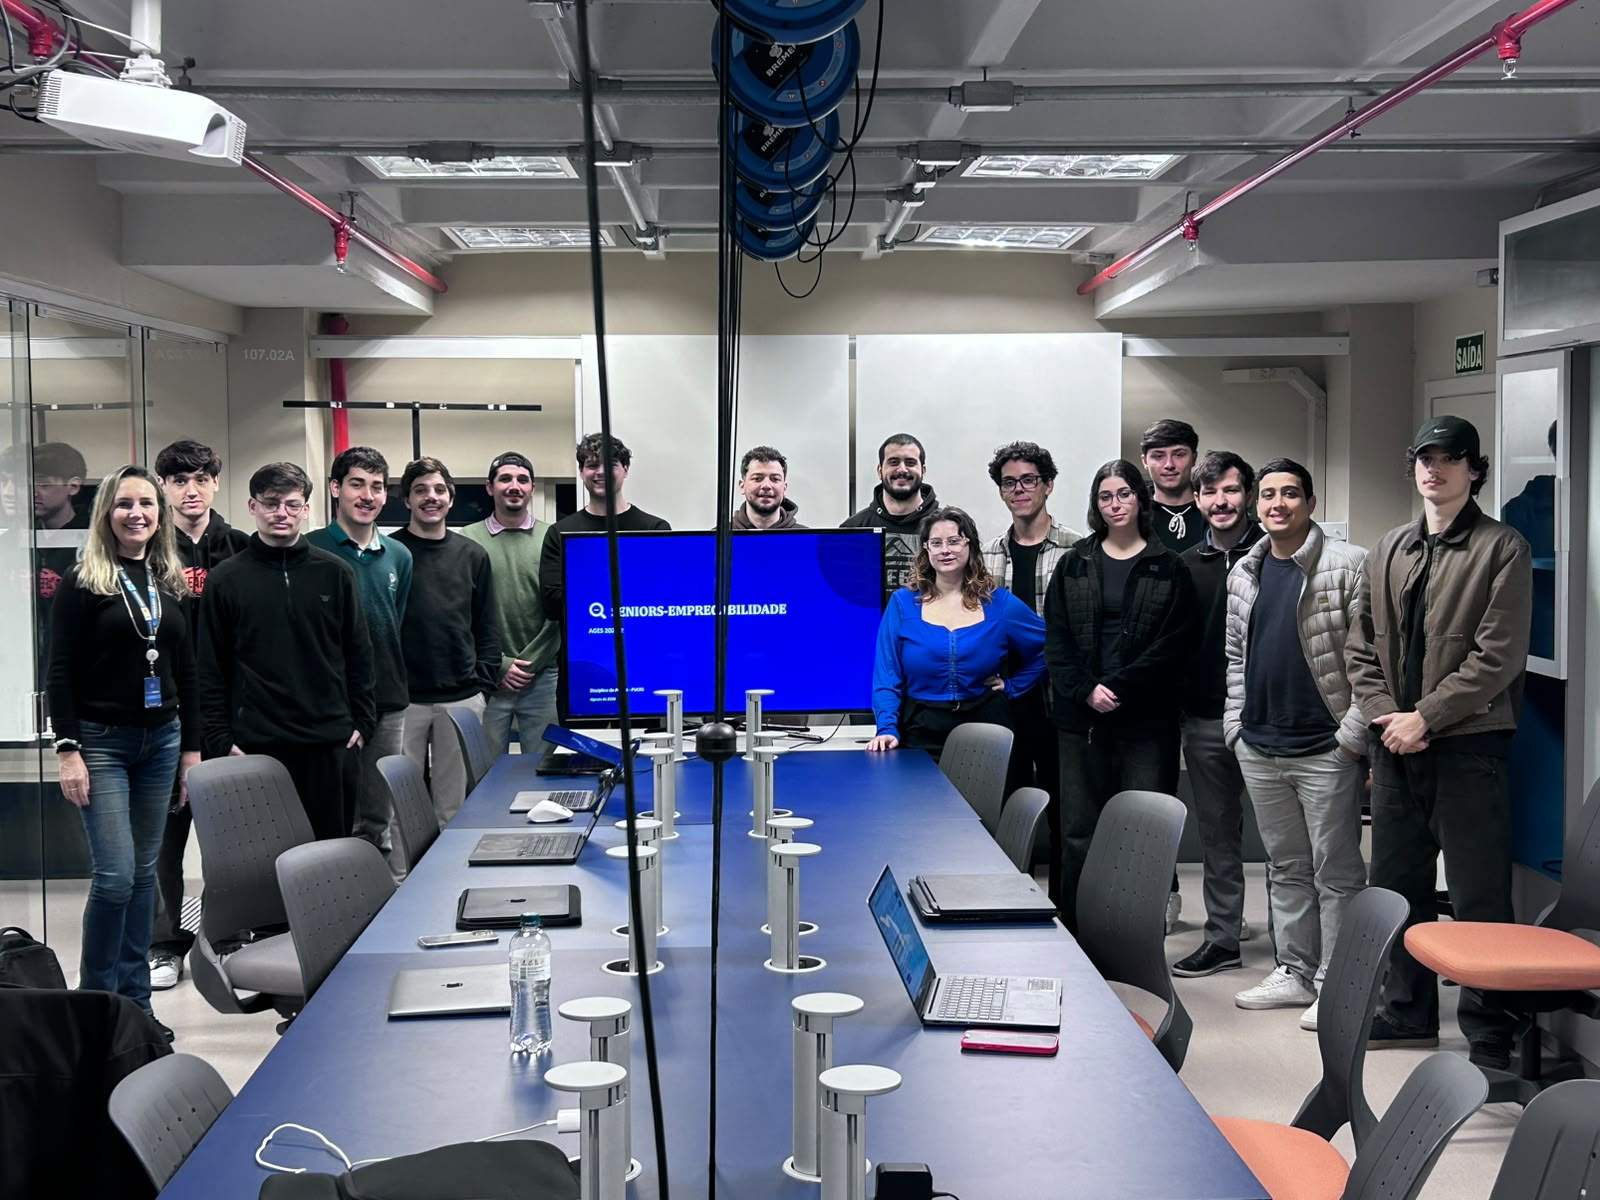
\includegraphics[width=1\linewidth]{conteudo/5 - ages IV/figures/foto-time-ages-iv.jpg}
  Fonte: Autor
  \label{fig:projeto-time4}
\end{figure}
